% \documentclass[chaparabic,mmi,msc,10pt,single]{metu} 
\documentclass[chaparabic,mas,ms,12pt,oneandhalf,threejury]{metu}

% Change this
% is: Information Systems
% phd: PhD
\usepackage{appendix}
\usepackage{longtable}
\usepackage[pdftex]{hyperref}
\usepackage[all]{hypcap}
\usepackage{todonotes}
\graphicspath{ {./images/} }
\usepackage[figuresright]{rotating}
\usepackage{xy} 
\usepackage{booktabs}
\usepackage{pifont}
\usepackage{color}
\usepackage{listings}
\usepackage{pdfpages}
\usepackage{array}
% \usepackage{algorithm}
% \usepackage{algorithmic}

\usepackage{algorithm2e}
\usepackage{tabularx}

\usepackage{float}
\usepackage{caption}
\usepackage{lastpage}
\usepackage{afterpage}
\usepackage{lipsum}
\usepackage{adjustbox}
\usepackage{rotating}
\usepackage{pdflscape}
\usepackage{hypcap}
\usepackage{threeparttable}

% \usepackage{graphicx}
\usepackage{amsmath,amssymb} % define this before the line numbering.
% \usepackage{ruler}
\usepackage{color}
% \usepackage{cite}
% \usepackage[utf8x]{inputenc}
% \usepackage{footnote}
% \makesavenoteenv{tabular}
% \makesavenoteenv{table}

\renewcommand{\sectionautorefname}{\S}
\renewcommand{\subsectionautorefname}{\S}

\newcommand{\norm}[1]{\left\lVert#1\right\rVert}

\captionsetup{belowskip=12pt,aboveskip=8pt}
\newcommand{\tab}{\hspace*{2em}}
\DeclareGraphicsExtensions{.pdf,.png,.jpg}
\DeclareCaptionLabelFormat{continued}{#1~#2 (Continued)}

\usepackage{amsmath}
\usepackage{siunitx}
\usepackage{textcomp}
\usepackage{subcaption}


\usepackage{tikz}
\usepackage{mathtools}
%\usepackage{rotating}
%\PassOptionsToPackage{figuresright}{rotating}

\DeclarePairedDelimiter\ceil{\lceil}{\rceil}
\DeclarePairedDelimiter\floor{\lfloor}{\rfloor}
\usepackage{multirow}
\usepackage{hvfloat}

\newcommand{\EA}[1]{\textcolor{red}{[EA: #1]}}

% Name and Surname
\author{Ayberk Aydin} % Change this
% Thesis Title English and Turkish
\title{IMPROVING PERCEPTUAL QUALITY OF SPATIALLY TRANSFORMED ADVERSARIAL EXAMPLES} % Change this
\turkishtitle{UZAMSAL DÖNÜŞÜMLÜ ÇEKİŞMELİ ÖRNEKLERİN ALGISAL KALİTESİNİN İYİLEŞTİRİLMESİ} % Change this

\date{August 2022} % Change this

 
% prof : Prof. Dr.
% assocprof : Assoc. Prof. Dr.
% assistprof : Assist. Prof. Dr.
% dr : Dr.
%
% Director of Institute
\director[prof]{Deniz Zeyrek Bozşahin} % Change this
% Head of Department
\headofdept[assocprof]{Elif Sürer} % Change this
%
% Supervisor : English and Turkish
\supervisor[prof]{Alptekin Temizel} % Change this
% \turkishsupervisor{  } %if you will hard-code the academic title
%
% Affiliation of Supervisor in English and possibly in Turkish
\departmentofsupervisor{Graduate School of Informatics, Middle East Technical University} % Change this

% \cosupervisor[assocprof]{Co-supervisor if Exists} % Change this
% \departmentofcosupervisor{Department, School} % Change this

% Committee Members
% In general members are sorted according to their academic titles
%
% Proffesors (1)
% Associate Professors (2)
% Assistant Professors (3)
% Other (4)
% 
% IMPORTANT:  All affiliatons should fit in a single line
% If affiliation line is broken into two lines you should shorten the affiliation by using 
% abbrevations or any other means
%
% First committee member should be the chair of examining committee
% Typically the chair is one of the highest ranked committee members
% Ask your supervisor if you are not sure
\committeememberi[prof]{Alptekin Temizel} % Change this
\affiliationi{Graduate School of Informatics, Middle East Technical University} % Change this
% Second committee member is always your supervisor
\committeememberii[assocprof]{Elif Sürer} % Change this
\affiliationii{Graduate School of Informatics, Middle East Technical University} % Change this

\committeememberiii[assocprof]{Gökhan Koray Gültekin} % Change this
\affiliationiii{Electrical\&Electronics Engineering, Ankara Yildirim Beyazit University}  % Change this
% If you are an M.Sc. student and your Co-Supervisor is in your 
% examination committee, then third committee member is always your co-supervisor
%
% IMPORTANT: If you are Ph.D. student your co-supervisor can not be in your 
% examination committee.

% \def\@proftitlename{Prof. Dr.}\def\@tproftitlename{Prof. Dr.}
% \def\@assocproftitlename{Assoc. Prof. Dr.}\def\@tassocproftitlename{Doç. Dr.}
% \def\@assistproftitlename{Assist. Prof. Dr.}\def\@tassistproftitlename{Yrd. Doç. Dr.}
% \def\@drtitlename{Dr.}\def\@tdrtitlename{Dr.}

% Fourth committee member
% \committeememberiv[assistprof]{Committee Member 4} % Change this
% \affiliationiv{Department, School} % Change this
% % Fifth committee member
% \committeememberv[assistprof]{Committee Member 5} % Change this
% \affiliationv{Department, School} % Change this
%
% Keywords : English & Turkish, Comma seperated
\keywords{deep learning, adversarial examples, perceptual quality} % Change this
\anahtarklm{derin öğrenme, çekişmeli örnekler, algısal kalite} % Change this
%
% Abstract in English
%
\abstract{
 Deep neural networks are known to be vulnerable to additive adversarial perturbations. The amount of these additive perturbations are generally quantified using \(\mathcal{L}_p\) metrics over the difference between adversarial and benign examples. However, even when the measured perturbations are small, they tend to be noticeable by human observers since \(\mathcal{L}_p\) distance metrics are not representative of human perception. Spatially transformed examples work by distorting pixel locations instead of applying an additive perturbation or altering the pixel values directly, which produces adversarial examples with improved visual quality. However, the perturbation made by spatial transformations produce visible non-smooth distortions on luminance channels and needs a smoothness regularization over the applied flow field in order to improve the visual quality. On the other hand, humans are less sensitive to changes in chrominance component of visual media and such as resolution loss or pixel shifts in a constrained neighborhood. Motivated by these observations, we propose a novel variation of spatially transformed adversarial examples that creates adversarial examples by applying spatial transformations to chrominance channels of perceptual colorspaces such as \(YC_{b}C_{r}\) and \(CIELAB\) to generate adversarial examples with high perceptual quality. Moreover, we find that the visual quality of these examples could be further improved by limiting the magnitude of applied spatial transformations. In a targeted white-box attack setting, the proposed method is able to obtain competitive fooling rates and experimental evaluations show that the proposed method has favorable results in terms of approximate perceptual distance between benign and adversarial images. 
} % Change this
%
% Turkish Abstract
%
\oz{
  Derin yapay sinir ağlarının eklemeli çekişmeli bozulmalara karşı savunmasız olduğu bilinmektedir. Bu bozulmaların miktarı \(\mathcal{L}_p\) metrikleri ile ölçülmektedir. Ancak, ölçülen bozulmaların miktarı az olsa da bu bozulmalar insan gözlemciler tarafından görülebilmektedir çünkü \(\mathcal{L}_p\) uzaklık metrikleri insan görüsünü yansıtmamaktadır. Uzamsal dönüşümlü örnekler piksel değerlerini doğrudan değiştirmek yerine piksel konumlarında bozulmalar yaparak görsel kalitesi yüksek çekişmeli örnekler üretir. Ancak, uzaysal dönüşümler tarafından yapılmış bozulmalar da parlaklık kanalında insanlar tarafından görülebilen pürüzsüz olmayan bozulmalara sebep olduğundan, bu yöntem görsel kaliteyi artırmak için bir pürüzsüzlük düzenlemesine ihtiyaç duymaktadır. Diğer yandan, insan görüsü görsel medyalardaki renk bileşeninin değişimine parlaklık değişiminden çok daha az duyarlıdır. Ayrıca kısıtlandırılmış komşuluklarda çözünürlük kaybı ve piksel kaymaları güçlükle fark edilebilmektedir. Bu çokluortam sıkıştırma gözlemlerinden yola çıkarak uzaysal dönüşümlü çekişmeli örneklerin \(YC_{b}C_{r}\) ve \(CIELAB\) gibi algısal renk uzaylarının renk bileşenlerine uzaysal dönüşüm yapan ve görsel kalitesi yüksek çekişmeli örnekler çıkaran yeni bir varyasyonu önerilmiştir. Buna ek olarak, uzaysal dönüşümün büyüklüğünü sınırlayarak görsel kalitenin daha da artırıldığı gözlemlenmiştir. Hedefli beyaz-kutu kurulumunda, önerilen yöntem yüksek bir güven puanı ile rekabetçi bir yanıltma oranı yakalamaktadır. Deneysel değerlendirilmeler, önerilen yöntemin, zararsız ve çekişmeli örnekler arasındaki algısal uzaklık cinsinden tercih edilir sonuçlar ortaya çıkardığını göstermektedir. 
} % Change this
%
% Dedication 
\dedication{
  To everyone
} % Change this
%
%
% Acknowledgements   
\acknowledgments{ This work has been funded by The Scientific and Technological Research Council of Turkey, ARDEB 1001 Research Projects Programme project no: 120E093 } % Change this
%
% End of Personal and Introductory Information
%%%%%%%%%%%%%%%%%%%%%%%%%%%%%%%%%5
\begin{document}
% Preliminaries
\begin{preliminaries}
  % If you are willing to use any custom stuff before Chapters, put it here
  % Such as List of Abbreviations
  % Check the abbreviations.tex for a template list of abbreviations

  \begin{theglossary}{LONGESTABBRV}

    \item[DNN] Deep Neural Network
    \item[ANN] Artifical Neural Network
    \item[CNN] Convolutional Neural Network
    \item[VIT] Vision Transformer
    \item[JPEG] Joint Photographic Experts Group
    \item[CIE] International Commission on Illumination
    \item[VGG] Visual Geometry Group
    \item[AI] Artifical Intelligence
    \item[DL] Deep Learning
    \item[NIPS] Conference on Neural Information Processing Systems
    \item[StAdv] Spatially Transformed Adversarial Examples
    \item[GPU] Graphics Processing Unit
    \item[RAM] Random Access Memory
    \item[VRAM] Video RAM
    \item[FGSM] Fast Gradient Sign Method
    \item[PGD] Projected Gradient Descent
    \item[BIM] Basic Iterative Method
    \item[C\&W] Carlini \& Wagner
    \item[TV] Total Variation
    \item[CAPTCHA] Completely Automated Public Turing Test to Tell Computers and Humans Apart
    \item[YUV] YUV color space - Y stands for luminance component and U and V stands for chrominance components
    \item[YCbCr] YCbCr color space - Y stands for luminance component and Cb and Cr stands for chrominance components
    \item[CIELAB] L*a*b* color space - L* stands for luminance component and a* and b* stands for chrominance components
    \item[LPIPS] Learned Perceptual Image Patch Similarity
    \item[SSIM] Structural Similarity Index Measure
    \item[MS-SSIM] Multi Scale Structural Similarity Index Measure
    \item[DISTS] Deep Image Structure and Texture Similarity
    \item[BFGS] Broyden-Fletcher-Goldfarb-Shannon Algorithm
    \item[L-BFGS] Limited Memory BFGS
    \item[HVS] Human Visual System
    \item[CUDA] Compute Unified Device Architecture


\end{theglossary}

  % End of Preliminaries
\end{preliminaries}
%   
% Latex content Goes Here 
% 
%

\setlength{\parindent}{0em}
\setlength{\parskip}{10pt}

% You can add as many chapters
% Change this
% CHAPTER 1
\chapter{Introduction}
\label{chp:1_introduction}

\section{Motivation and Problem Definiton}
In recent years, deep neural networks have shown impressive performance in many vision related tasks such as image classification~\cite{he2015deep}, object detection~\cite{redmon2018yolov3} and image segmentation~\cite{long2015fully}. However, they are found to be vulnerable to intentionally crafted small perturbations called adversarial perturbations~\cite{szegedy2013intriguing}. These small perturbations added to the input image successfully change the output of a trained classifier by altering the logits large enough to change its decision to a preferred class~\cite{goodfellow2014explaining}. While these perturbations are optimized in \(\mathcal{L}_p\) spaces~\cite{carlini2017towards}, they are visible to human observers, since small \(\mathcal{L}_p\) does not always correspond to perturbations with less perceptual distortion~\cite{jordan2019quantifying,engstrom2018rotation}. 

Since this intriguing property of neural networks has security implications in the production setting, it is often called as adversarial attacks. For example, websites are using Completely Automated Public Turing Tests to Tell Computers and Humans Apart (CAPTCHA) to prevent automated request agents such as web scrapers and spiders from automatically reaching their content. A widely used CAPTCHA is asking to select the images that is from a specific class such as "bicycle" or "crossroad" among the provided images. A human can effortlessly detect the suitable images while web scrapers need to use DNNs to classify each image and select the correct ones. A simple and widely modification for CAPTCHAs is distorting the content so that automated CAPTCHA solvers would fail the test without affecting humans. To do this, recent CAPTCHAs has extended this setup by adding adversarial perturbations to the provided images to prevent DNN classified based solvers from automatically selecting the correct images. In Figure \ref{fig:googlecaptcha}, a recent CAPTHCA from Google is shown where it is asked to select the images that contains "cars". Normally, a trained DNN could be used to classify images and to select the images whose output is the class "car" to pass the test. However, there is a noticeable adversarial noise added to the images to fool the DNN and to prevent the attacker from passing the test.
\begin{figure}[t]
    \centering
    \includegraphics[width=0.4\linewidth]{captchas/1.png}
    \includegraphics[width=0.4\linewidth]{captchas/2.png}
    \caption{Two CAPTCHA examples from Google where adversarial examples are used to prevent web scrapers and spiders that are using automatic image classifiers such as DNNs by adversarially perturbing the CAPTCHA images.}\label{fig:googlecaptcha}
\end{figure}

A serious risk of 


Multimedia compression standards have been developed to compress visual multimedia such as images and videos to reduce the amount of data with minimum amount of distortion to the perceived output. One of the most fundamental findings about human vision that most lossy visual multimedia compression methods utilise is that human vision is much less sensitive to the information loss in color than the luminance.
%evolution%
This observation is utilized in image compression as a technique known as ``chroma subsampling''. There are variants of chroma subsampling that only subsamples chrominance along horizontal axis (4:2:2) or both horizontal and vertical axes (4:2:0). Without further compression, (4:2:0) chroma subsampling reduces the size of an image effectively to half of its original size. Replacing the chroma components of the pixels in by neighboring chroma components does not yield visible artifacts.
\section{Proposed Methods}
We employ these observations to derive a new type of adversarial attack based on spatial transformations in chroma channels of perceptual colorspaces. We apply spatial transformation only to the chroma components of input image while keeping the luminance component intact. Figure~\ref{fig:flowtochannels} shows the effect of a randomly initialized flow field applied to the luminance, chrominance and both set of channels. It is clear that spatial transformation in luminance channels causes visible distortions while chrominance only spatial transformations cause very subtle changes for human vision. This effect is much more highlighted when only the differences are observed after applying a flow field. Figure \ref{fig:outofgamut} shows the absolute pixel difference from the initial image when the same flow field is applied to RGB, \(C_{b}C_{r}\) and a*b* channels, respectively.
\begin{figure}[t]
    \centering
    \begin{subfigure}[b]{.30\linewidth}
        \includegraphics[width=\linewidth]{img.png}
        %        \caption{Original}
        \caption{}
    \end{subfigure}
    \begin{subfigure}[b]{.30\linewidth}
        \includegraphics[width=\linewidth]{flowed_cbcr.png}
        %        \caption{Flow to CbCr channels}
        \caption{}
    \end{subfigure}
    \begin{subfigure}[b]{.30\linewidth}
        \includegraphics[width=\linewidth]{flowed_ab.png}
        %       \caption{Flow to \(a^*b^*\) channels}
        \caption{}
    \end{subfigure}
    \begin{subfigure}[b]{.30\linewidth}
        \includegraphics[width=\linewidth]{flowed_rgb.png}
        %      \caption{Flow to RGB channels}
        \caption{}
    \end{subfigure}
    \begin{subfigure}[b]{.30\linewidth}
        \includegraphics[width=\linewidth]{flowed_y.png}
        %     \caption{Flow to Y channel}
        \caption{}
    \end{subfigure}
    \begin{subfigure}[b]{.30\linewidth}
        \includegraphics[width=\linewidth]{flowed_l.png}
        %\caption{Flow to L channel}
        \caption{}
    \end{subfigure}
    \caption{Effect of flow field applied to different channels, (a) original image, Images where flow field is applied to (b) \(C_{b}C_{r}\), (c) \(a^*b^*\), (d) RGB, (e) Y and (f) L channel. The magnitude of the flow is scaled up to emphasize the effect for illustration.}\label{fig:flowtochannels}
\end{figure}

\begin{figure}[t]
    \centering
    \begin{subfigure}[b]{.4\linewidth}
        \includegraphics[width=\linewidth]{diff/209_lab_adv.png}
        \caption{}
    \end{subfigure}
    \begin{subfigure}[b]{.4\linewidth}
        \includegraphics[width=\linewidth]{diff/209_rgb_diff.png}
        \caption{RGB}
    \end{subfigure}
    \begin{subfigure}[b]{.4\linewidth}
        \includegraphics[width=\linewidth]{diff/209_ycbcr_diff.png}
        \caption{a*b*}
    \end{subfigure}
    \begin{subfigure}[b]{.4\linewidth}
        \includegraphics[width=\linewidth]{diff/209_lab_diff.png}
        \caption{CbCr}
    \end{subfigure}
    \caption{Visual difference from random flow field application to different channels, (a) original image, Visualization of pixel differences where flow field is applied to (b) RGB, (c) \(C_{b}C_{r}\), (d) \(a^*b^*\) channels. The magnitude of the flow is scaled up and contrast of the pixel differences is increased to increase the visibility for illustration. }\label{fig:diff}
\end{figure}


\section{Contributions of the Study}

The main findings of this thesis is published in a paper~\cite{aydin2019imperceptible} and the subject is further elaborated in this thesis. The contributions of this work can be summarized as following;
\begin{itemize}
    \item Utilization of the findings of human vision and ideas from multimedia compression to make imperceptible changes on images without any \(L_p\) norm restriction or regularization.
    \item A novel method to generate adversarial examples with little to no perceptual distortion by applying spatial transformations in chroma channels of perceptual colorspaces.
    \item Colorfulness analysis of NIPS2017 Adversarial Challenge dataset.
\end{itemize}

\section{Organization of the Thesis}
This thesis is organized as follows. Chapter \ref{chp:1_introduction} provides an introduction on the thesis topic, explaining the motivation, defines the problem attacked and briefly explains the methods and contributions of the thesis. Chapter \ref{chp:2_literature} mentions the literature about the thesis topic, presents the types and classifications of adversarial attacks and methods for generating imperceptible types of adversarial attacks or methods to improve perceptual quality of adversarial examples. Chapter \ref*{chp:3_methodology} explains the methodology of the method proposed in this thesis in a detailed manner. It starts with spatial transformations, then explains spatially transformed adversarial examples and colorspaces to build the foundation of this thesis. Then, it explains the method proposed in this thesis. Chapter \ref{chp:4_results} mentions the setup of the experiments and presents the experimental results. Chapter \ref{chp:5_discussion} provides a discussion about the results presented in Chapter \ref{chp:5_discussion}, explains the implications of the results and mentions the failure cases, discussing the possible reasons. Chapter \ref{chp:6_conclusion} draws conclusions on the thesis along with possible future studies of the new research questions with the thesis.


\chapter{related work}
\label{chp:2_literature}

In this chapter, related studies are given in detail. Firstly, the concept of adversarial examples and the types of adversarial examples are explained briefly. Then, spatially transformed adversarial examples are explained in detail.
\section{Adversarial Examples}

The concept of adversarial examples were introduced by Szegedy et al.~\cite{szegedy2013intriguing}. They found that adding small calculated perturbances to the input image is able to change the decision of the target classifier (deep neural network) without affecting the decision human observers. Even though the perturbation is small, it can be easily noticed by human observers by "visual noise" instead of semantically meaningful patterns. Since this intriguing property of neural networks has security implications in the production setting, it is often called as adversarial attacks. For example, websites are using Completely Automated Public Turing Tests to Tell Computers and Humans Apart (CAPTCHA) to prevent web scrapers and spiders from automatically reaching their content. A widely used CAPTCHA is asking to select the images that is from a specific class such as "bicycle" or "crossroad" among the provided images. A human can effortlessly detect the suitable images while web scrapers need to use DNNs to classify each image and select the correct ones. Recent CAPTCHAs has extended this setup by adding adversarial perturbations to the provided images to prevent DNNs from automatically selecting the correct images. In Figure \ref{fig:googlecaptcha}, a recent CAPTHCA from Google is shown where it is asked to select the images that contains "cars". Normally, a trained DNN could be used to classify images and to select the images that outputs the class "car" to pass the test. However, there is a noticable adversarial noise added to the images to fool the DNN and to prevent the scraper from passing the test.
\begin{figure}[t]
    \centering
    \includegraphics[width=0.4\linewidth]{captchas/1.png}
    \includegraphics[width=0.4\linewidth]{captchas/2.png}
    \caption{Two CAPTCHA examples from Google where adversarial examples are used to fool web scrapers and spiders that are using automatic image classifiers such as DNNs.}\label{fig:googlecaptcha}
\end{figure}

Adversarial attacks can be classified as white-box and black-box depending on whether the attacker could reach the neural network parameters and gradients or not, respectively. Also, they can be classified as targeted or untargeted attacks. In targeted attack setup, there exists a particular class that attacker tries to modify the input image to have the attacked neural network to output that particular class and considered successful (or fooled the network) if the network outputs the target class when fed with the modified adversarial example. On the other hand, in the untargeted attack setting the attacker modifies the image to prevent the neural network from deciding the true class, which is the ground truth label of the input image and considered successful if the network outputs a class other than the true class label. In this thesis, targeted white-box attack setup is used. Other than the decision of the target network, there is often a magnitude constraint to the perturbation made and \(\mathcal{L}_p\) norms are widely used to measure the magnitude of the added perturbation. Adversarial attacks can be formally defined as a constrained optimization problem where the attacker tries to maximize a loss function by perturbing the input while the magnitude of the perturbation is constrained. Generally, the adversarial loss is the loss that is minimized throughout the training process. In most general form, the optimization process can be formulated as Equation \ref{eqn:somelabel}

\begin{equation}
    \label{eqn:somelabel}
    e=mc^2
\end{equation}

They also proposed a simple technique to generate adversarial examples called Fast Gradient Sign Method~(FGSM). It works by first calculating the gradient of the input with respect to a loss function, which is generally cross entropy loss

\section{Colorspaces}

\section{Perceptual Quality Preserving Adversarial Attacks}
Utilizing perceptual colorspaces and metrics for imperceptible adversarial example generation is investigated in several studies. Aksoy et al. investigated additive noise based attacks on chrominance channels in YUV colorspace \cite{aksoy2019attack}, which is the analog counterpart of \(YC_{b}C_{r}\) space. Despite Pestana et al. found that adversarial perturbations are more highlighted in luminance channels in terms of the magnitude~\cite{Pestana2020-hm}, Aksoy et al. found that even suppressing the luminance perturbation, additive noise based attack on chrominance channels still successfully fool target networks, yet causes visible distortion. In our earlier work, we also explored spatial transformations to UV channels of YUV to generate imperceptible adversarial examples~\cite{aydin2019imperceptible} and we extend this work by exploring \(YC_{b}C_{r}\) space as well as perceptually uniform CIELAB space and measuring structured similarity metrics such as SSIM~\cite{wang2004image} and MS-SSIM~\cite{wang2003multiscale} between benign images and adversarially generated images. Karli et al. leveraged perceptual metric LPIPS~\cite{zhang2018unreasonable} to improve the quality of adversarial examples. Since LPIPS is a differentiable metric, they used gradient based optimization to minimize LPIPS alongside the adversarial loss. Similarly, Zhao et al. replaced CIEDE2000 perceptual distance metric~\cite{luo2001development} with \(\mathcal{L}_{p}\) norm constraint in Carlini \& Wagner attack to produce perceptually close adversarial examples.

\section{Spatially Transformed Adversarial Examples}

Spatial transformations as a method for generating adversarial examples was first proposed in ~\cite{xiao2018spatially}, where it is shown that small displacements applied to input pixels can successfully fool a target network. However, using this method, even small displacements could cause visible distortions when the adjacent pixels are drifted towards different directions. As a remedy to this problem, use of  Total Variation~(TV) regularization~\cite{estrela2016total} was proposed. Application of TV regularization to the flow field pushes the neighboring displacement vectors to the same direction and, hence, produces smoother output. Similarly, Jordan et al. combined spatial transformations with \(l_\infty\) bounded attacks to forge stronger attacks with better perceptual quality. Croce et al. argued adding noise to smooth areas of an image causes visible artifacts and proposed "hiding" the perturbations at the locations with high spatial variations such as edges and corners~\cite{croce2019sparse}. As seen from Figure \ref{fig:diff}, perturbations made with our method naturally occurs in the places with high variations since it is based on local spatial transforms.



Unlike these methods, the attack proposed in this paper does not rely on auxiliary losses or explicit perceptual distance terms in optimization process to produce examples with high perceptual quality. In addition, it does not require regularization, unlike spatial transformation based methods such as ~\cite{xiao2018spatially}, due to its intrinsic imperceptibility. It should be noted that the existing spatial transformation based methods, as well as our work, does not utilize limited degree of freedom transformations such as rotation, translation or scaling that can be formulated as a \(4\times4\) transformation matrix~\cite{jaderberg2015spatial}. In that formulation, the flow field \(f \in \mathbb{R}^{2\times H \times W}\) is calculated using the transformation matrix. Instead, we directly define and optimize flow field, where the number of parameters is equal to twice number of pixels in the input image since there is an x and y component for each pixel. Application and optimization of flow field is explained in the Section \ref{chp:3_methodology}.


\chapter{Methodology}
\label{chp:3_methodology}
In this work, we address the problem of creating targeted adversarial examples without adversarial perturbation being perceptible by human vision. For this purpose, we use a modified version of Spatially Transformed Adversarial Examples~\cite{xiao2018spatially} that perturbs the input image only in the channels that human vision is not sensitive to the spatial information loss in \(YC_{b}C_{r}\) and CIELAB colorspace representations of the input image. 

\section{Proposed Method}

The proposed adversarial example generation method is as follows. Let \(x \in \mathbb{R}^{3\times H \times W}\) be the 3-channel input image, where \(H, W\) are the height and the width of the image, respectively. First, we randomly initialize a flow field \(f \in \mathbb{R}^{2\times H \times W}\) where a two-dimensional vector exists for each pixel location of the adversarial image \(x_{adv}\). Then, we apply the flow field to the benign image as explained below to obtain the adversarial image. Then, we feed the adversarial image to the target network and backpropagate the loss gradient to the flow field. Since the flow field application is a differentiable process, it can be optimized by stochastic gradient descent and variants such as Adam~\cite{kingma2015adam} or L-BFGS\cite{liu1989limited}. The optimization process is repeated until the attack is successful or the maximum iteration count is reached. Visual illustration of the adversarial image generation methodology is shown in Figure~\ref{fig:algorithm}

\begin{figure*}[t]
    \centering
    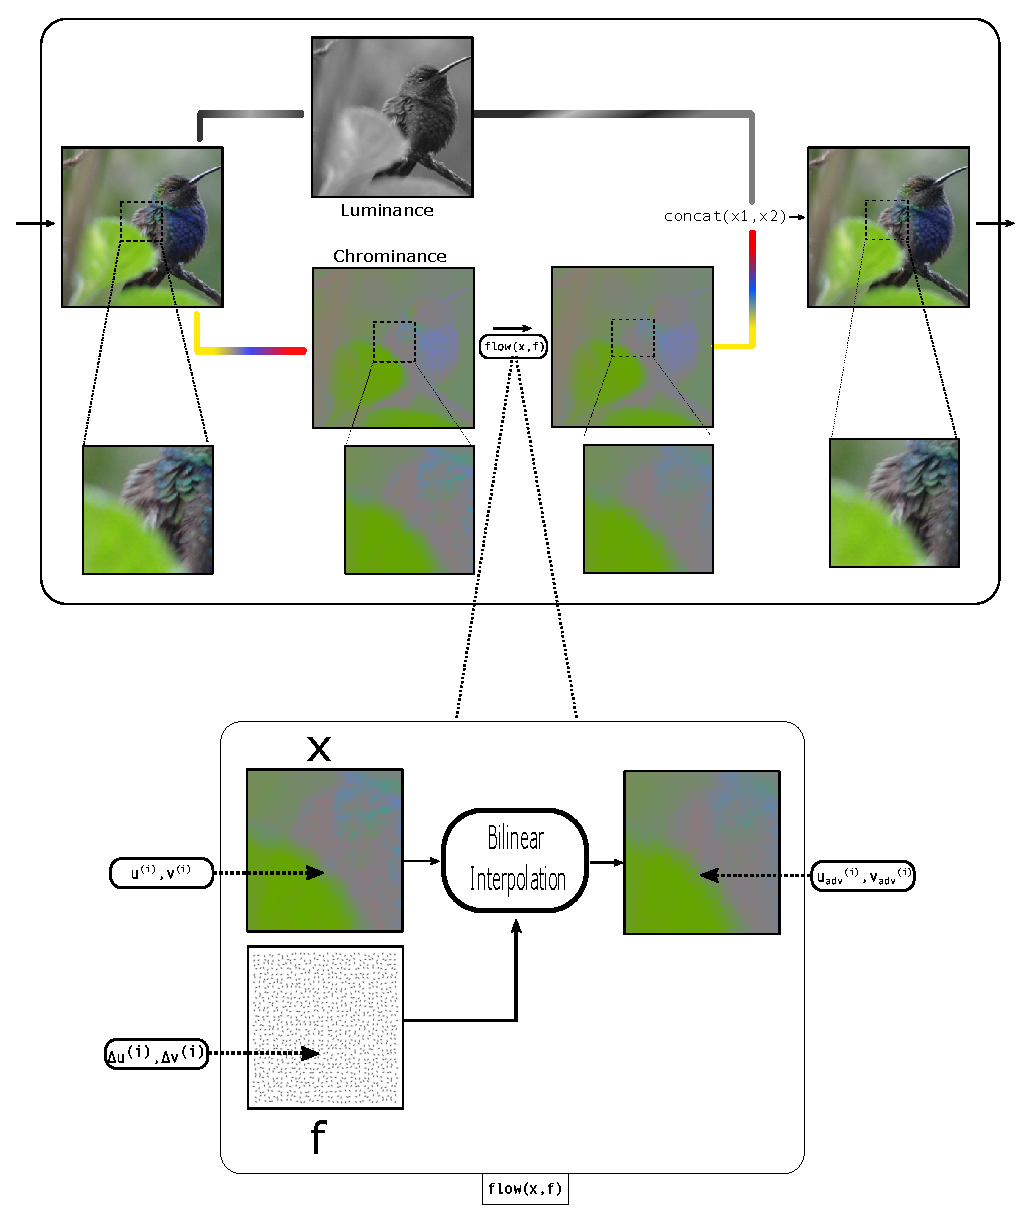
\includegraphics[width=0.8\linewidth]{illustration/drawing.eps}
    \caption[Visual illustration of the proposed adversarial example generation method.]{Visual illustration of the proposed adversarial example generation method. Luminance and chrominance channels are Y and \(C_{b}C_{r}\) when \(YC_{b}C_{r}\) colorspace and L and \(a^*b^*\) when CIELAB colorspace is used. Visual representation of flow field, subpixel restriction by \(\tanh\) and conversion of concatenated image back to RGB colorspace is omitted for brevity.}\label{fig:algorithm}
\end{figure*}

\RestyleAlgo{ruled}
\begin{algorithm}[t]
    \caption{Adversarial example generation by spatial transformation in chrominance channels in a perceptual colorspace. }\label{alg1}
    \KwIn{   \(x\)

    }
    \KwOut{   \(x_{adv}\)}
    \KwData{
        target\_class,
        model,
        \(\kappa\),
        colorspace,
        max\_iters,
        is\_restricted,
    }
    \(f \sim \mathcal{N}(0,\,\sigma^{2})\)\;
    \(i \gets 0\);

    \While{\(i < max\_iters\)}{
    \If{\(colorspace == YC_{b}C_{r}\)}{
    \(x_{color} \gets to\_ycbcr(x)\)\;
    }
    \If{\(colorspace == CIELAB\)}{
        \(x_{color} \gets to\_lab(x)\)\;
    }
    \(x_{luma}, x_{chroma} \gets splitchannels(x_{color})\)\;
    \If{is\_restricted}{\(f \gets \tanh(f)\)}
    \(x_{chroma} \gets apply\_flow(x_{chroma}, f)\)\;
    \(x_{adv} \gets concat(x_{luma}, x_{chroma})\)\;
    \(x_{adv} \gets to\_rgb(x_{adv})\)\;
    \(adv\_scores = model(x_{adv})\)\;
    \(loss \gets loss\_fn(adv\_scores, target\_class, \kappa)\)\;
    \eIf{\(loss \leq \kappa\)}
    {\Return{\(x_{adv}\)}\;}
    {

        \(backprop(loss)\)\;
        \(update(f)\)\;
        \(i \gets i + 1\)\;
    }
    }
\end{algorithm}

\subsection{Application of flow field}
Flow field is applied to the benign image following the methodology in~\cite{xiao2018spatially} also explained in Chapter~\ref{chp:2_literature}. For each pixel in adversarial image \(i_{adv}\), corresponding flow field vector value \(p_{i,j}\) is added to the pixel location. Then, the corresponding pixel at the added location is sampled. Since the added location is not an integer, bilinear interpolation is used to sample from the fractional pixel locations. Bilinear interpolation also makes the method end-to-end differentiable, thus optimizable by gradient based optimizers.
%\subsubsection{Restricting the flow field}
Chroma subsampling effectively causes the same chroma values to be used by the neighboring pixels, and it is widely accepted to cause negligible changes to the images. Accordingly, to exploit this fact, we can impose a restriction to the flow field to keep its values in the range \((-1, 1)\). We initialize a pre-flow field \(f_{pre}\) and calculate the applied flow field as \(f = \tanh(f_{pre})\). This differentiable reparameterization~\cite{mordvintsev2018differentiable} of flow field constraints the flow field magnitude to be smaller than 1 without inhibiting end-to-end differentiability so that chrominance value of each pixel of the adversarial image \(x_{adv}\) is only affected by the value of the pixel of the same location in \(x\) and its neighboring pixels. %With this modification, chroma subsampling becomes a very effective defense method to the subpixel restricted variant our attack without making any visually perceptible changes, as discussed in Section~\refeq{section:discussion}.
To make the adversarially perturbed images indistinguishable from their benign counterparts, the flow field is applied only to the channels that human vision is not very sensitive to~\cite{vorobyev2004ecology}. Since widely used RGB colorspace is not designed to be a perceptual colorspace, even small spatial perturbations to any RGB channel creates visually distinguishable changes. Hence, we first convert the benign image to a perceptual colorspace such as \(YC_{b}C_{r}\) where human vision is not sensitive to the spatial perturbations in, which is \(C_{b}\) and \(C_{r}\) in \(YC_{b}C_{r}\), and \(a^*\) and \(b^*\) in CIELAB colorspace. Then, we apply the flow field only to the channels Cb and Cr in \(YC_{b}C_{r}\), and A and B in CIELAB colorspace.


% In many multimedia compression standards such as JPEG and MPEG, chroma components are usually subsampled to compress information without making visually perceptible changes.



\chapter{Experiments}
\label{chp:4_results}
\section{Dataset}

We used the dataset and the provided model from NIPS 2017 Competition on Adversarial Attacks and Defenses~\cite{kurakin2018adversarial} to evaluate our method. NIPS 2017 dataset is a collection of 1000 images curated by Google Brain with the resolution of \(299 \times 299\) with their corresponding true and target classes from Imagenet~\cite{deng2009imagenet} dataset. For the target network, we used Inception-v3~\cite{szegedy2016rethinking} architecture and Imagenet trained checkpoint provided with the dataset.
\section{Experimental Evaluation}
We conducted our experiments in a white-box setup where the gradients are fully available. Experiments have been done in a targeted attack setting with the dataset provided targets. We optimized using Adam~\cite{kingma2015adam} with the default settings and used Carlini \& Wagner loss~\cite{carlini2017towards} with confidence margin \(\kappa \in \left\{ 0, 10 \right\}\).



%\subsection{Results}
%\subsection{Fooling Rate and Success Rate}
We compared the success rate of our attack in CIELAB and \(YC_{b}C_{r}\) against stAdv in both restricted and unrestricted settings. An attack is considered successful if the Carlini \& Wagner loss is less than \(-\kappa\). We did not use the smoothness regularization term in stAdv for a fair comparison.
\begin{table}[t]
    \caption{Attack success rates with \(\kappa = 0\) and \(\kappa = 10\) in not restricted and subpixel restricted settings for RGB, \(a^*b^*\) and \(C_{b}C_{r}\) attacks. }

    \begin{tabularx}{\linewidth}{ X  X  X  X }
        \toprule
                                               & RGB                   & \(C_{b}C_{r}\)        & \(a^{*}b^{*}\)        \\
        \hline
        \multicolumn{4}{c}{Not Restricted}                                                                             \\
        \midrule
        \(\kappa\) = 0\newline \(\kappa\) = 10 & 100\%\newline 100\%   & 95.0\%\newline 83.8\% & 95.7\%\newline 87.3\% \\
        \hline
        \multicolumn{4}{c}{Restricted to Subpixel}                                                                     \\
        \midrule
        \(\kappa\) = 0\newline \(\kappa\) = 10 & 99.8\%\newline 99.7\% & 86.1\%\newline 47.0\% & 89.2\%\newline 53.2\% \\
        \bottomrule
    \end{tabularx}\label{table:foolingrate}
\end{table}


\begin{figure}[t]
    \begin{subfigure}[b]{\linewidth}
        \caption{}

        \includegraphics[width=0.24\linewidth]{examples/benign_0.png}
        \includegraphics[width=0.24\linewidth]{examples/example_lab_0.png}
        \includegraphics[width=0.24\linewidth]{examples/example_ycbcr_0.png}
        \includegraphics[width=0.24\linewidth]{examples/example_rgb_0.png}
    \end{subfigure}

    \begin{subfigure}[b]{\linewidth}
        \caption{}
        \includegraphics[width=0.24\linewidth]{examples/benign_4.png}
        \includegraphics[width=0.24\linewidth]{examples/example_lab_4.png}
        \includegraphics[width=0.24\linewidth]{examples/example_ycbcr_4.png}
        \includegraphics[width=0.24\linewidth]{examples/example_rgb_4.png}
    \end{subfigure}

    \begin{subfigure}[b]{\linewidth}
        \caption{}
        \includegraphics[width=0.24\linewidth]{examples/benign_5.png}
        \includegraphics[width=0.24\linewidth]{examples/example_lab_5.png}
        \includegraphics[width=0.24\linewidth]{examples/example_ycbcr_5.png}
        \includegraphics[width=0.24\linewidth]{examples/example_rgb_5.png}
    \end{subfigure}

    \ContinuedFloat
    \begin{subfigure}[b]{\linewidth}
        \caption{}
        \includegraphics[width=0.24\linewidth]{examples/benign_20.png}
        \includegraphics[width=0.24\linewidth]{examples/example_lab_20.png}
        \includegraphics[width=0.24\linewidth]{examples/example_ycbcr_20.png}
        \includegraphics[width=0.24\linewidth]{examples/example_rgb_20.png}
    \end{subfigure}

    \ContinuedFloat
    \begin{subfigure}[b]{\linewidth}
        \caption{}
        \includegraphics[width=0.24\linewidth]{examples/benign_7.png}
        \includegraphics[width=0.24\linewidth]{examples/example_lab_7.png}
        \includegraphics[width=0.24\linewidth]{examples/example_ycbcr_7.png}
        \includegraphics[width=0.24\linewidth]{examples/example_rgb_7.png}
    \end{subfigure}

    \begin{subfigure}[b]{\linewidth}
        \caption{}
        \includegraphics[width=0.24\linewidth]{examples/benign_30.png}
        \includegraphics[width=0.24\linewidth]{examples/example_lab_30.png}
        \includegraphics[width=0.24\linewidth]{examples/example_ycbcr_30.png}
        \includegraphics[width=0.24\linewidth]{examples/example_rgb_30.png}
    \end{subfigure}


    \caption{Examples from the dataset and adversarial examples generated with their target class probabilities from target network Inception-v3. From left to right; Benign image, adversarial image generated by attacking in  and RGB. }\label{fig:visualprob}
\end{figure}

\begin{table}[t]
    \caption{Average amount of distortion required to fool the target network with very high confidence (\(\kappa=10\)) in not restricted and subpixel restricted settings.}
    \label{table:perceptualmetrics}
    \begin{tabularx}{\linewidth}{ X  X  X  X }
        \toprule

                                           & RGB                               & \(C_{b}C_{r}\)                                             & \(a^*b^*\)                                \\
        \hline
        \multicolumn{4}{c}{Not Restricted}                                                                                                                                              \\
        \midrule
        LPIPS\newline SSIM\newline MS-SSIM & 0.327\newline 0.321\newline 0.164 & \textbf{0.019}\newline \textbf{0.067}\newline 0.017        & 0.022\newline 0.070\newline\textbf{0.016} \\
        \hline
        \multicolumn{4}{c}{Restricted to Subpixel}                                                                                                                                      \\
        \midrule
        LPIPS\newline SSIM\newline MS-SSIM & 0.222\newline 0.220\newline 0.037 & \textbf{0.012}\newline\textbf{0.050}\newline\textbf{0.011} & 0.014\newline 0.056\newline 0.013         \\
        \bottomrule
    \end{tabularx}
\end{table}
\subsection{Analysis of the Results}
Figure~\ref{fig:visualprob} shows the original images alongside with the adversarial images generated (with \(\kappa = 10\)) by attacking in \(a^*b^*\), \(C_{b}C_{r}\) and RGB spaces. As can be observed from these images, perceptual distortions are much less pronounced for chrominance-only attacks. Attacking in RGB domain, which is the default approach in the literature, results in modification of the luminance channels, leading to much more visible artifacts.

Table~\ref*{table:foolingrate} shows the attack success rates for attacks on different colorspaces. The results show that, adversarial images generated by attacks exclusively targeting the chrominance channels can fool the network with a high probability as well. On the other hand, they are less effective when restricted to operate in a subpixel-only setting. The fooling rate of a*b* attacks are slightly higher than \(C_bC_r\) attacks. We argue that this is due to many examples in the dataset being chroma subsampled in \(YC_bC_r\) space, as an indirect effect of image compression, restricting the search space for \(C_bC_r\) attacks.

We measured the amount of distortion required to generate confident (\(\kappa = 10\)) adversarial examples with the following perceptual metrics: Learned Perceptual Image Patch Similarity~(LPIPS) ~\cite{zhang2018unreasonable}, Structured Similarity Index~(SSIM) ~\cite{wang2004image} and Multi-Scale SSIM~(MS-SSIM) ~\cite{wang2003multiscale}. Table~\ref{table:perceptualmetrics} shows the average results over the successful attacks for each perturbation mode in terms of these metrics. Since SSIM and MS-SSIM are similarity metrics, values of \(1-\)SSIM and \(1-\)MS-SSIM are provided. Hence, for all metrics, lower values are better. According to these results, colorspace restricted attacks have much better scores in terms of perceptual metrics compared to RGB attacks, implying that there is significantly less perceptual difference between benign and adversarial examples. While \(C_bC_r\) attacks generally produce better images in terms of perceptual quality metrics than a*b* attacks, the difference is relatively low.

\chapter{Experiments}
\label{chp:5_discussion}
\section{Experimental Evaluation}
We conducted our experiments in a white-box setup where the gradients are fully available. Experiments have been done in a targeted attack setting with the dataset provided targets. We optimized using Adam~\cite{kingma2015adam} with the default settings and used Carlini \& Wagner loss~\cite{carlini2017towards} with confidence margin \(\kappa \in \left\{ 0, 10 \right\}\).

%\subsection{Dataset and Model} 

We used the dataset and the provided model from NIPS 2017 Competition on Adversarial Attacks and Defenses~\cite{kurakin2018adversarial} to evaluate our method. NIPS 2017 dataset is a collection of 1000 images curated by Google Brain with the resolution of \(299 \times 299\) with their corresponding true and target classes from Imagenet~\cite{deng2009imagenet} dataset. Alongside the dataset, an Imagenet trained Inception-v3~\cite{szegedy2016rethinking} model is provided. %Unless specified otherwise, results are reported using the dataset and model from NIPS2017 challenge.

%\subsection{Results}
%\subsection{Fooling Rate and Success Rate}
We compared the success rate of our attack in CIELAB and \(YC_{b}C_{r}\) against stAdv in both restricted and unrestricted settings. An attack is considered successful if the Carlini \& Wagner loss is less than \(-\kappa\). We did not use the smoothness regularization term in stAdv for a fair comparison.
\begin{table}[t]
    \caption{Attack success rates with \(\kappa = 0\) and \(\kappa = 10\) in not restricted and subpixel restricted settings for RGB, \(a^*b^*\) and \(C_{b}C_{r}\) attacks. }

    \begin{tabularx}{\linewidth}{ X  X  X  X }
        \toprule
                                               & RGB                   & \(C_{b}C_{r}\)        & \(a^{*}b^{*}\)        \\
        \hline
        \multicolumn{4}{c}{Not Restricted}                                                                             \\
        \midrule
        \(\kappa\) = 0\newline \(\kappa\) = 10 & 100\%\newline 100\%   & 95.0\%\newline 83.8\% & 95.7\%\newline 87.3\% \\
        \hline
        \multicolumn{4}{c}{Restricted to Subpixel}                                                                     \\
        \midrule
        \(\kappa\) = 0\newline \(\kappa\) = 10 & 99.8\%\newline 99.7\% & 86.1\%\newline 47.0\% & 89.2\%\newline 53.2\% \\
        \bottomrule
    \end{tabularx}\label{table:foolingrate}
\end{table}


\begin{table}[t]
    \caption{Average amount of distortion required to fool the target network with very high confidence (\(\kappa=10\)) in not restricted and subpixel restricted settings.}
    \label{table:perceptualmetrics}
    \begin{tabularx}{\linewidth}{ X  X  X  X }
        \toprule

                                           & RGB                               & \(C_{b}C_{r}\)                                             & \(a^*b^*\)                                \\
        \hline
        \multicolumn{4}{c}{Not Restricted}                                                                                                                                              \\
        \midrule
        LPIPS\newline SSIM\newline MS-SSIM & 0.327\newline 0.321\newline 0.164 & \textbf{0.019}\newline \textbf{0.067}\newline 0.017        & 0.022\newline 0.070\newline\textbf{0.016} \\
        \hline
        \multicolumn{4}{c}{Restricted to Subpixel}                                                                                                                                      \\
        \midrule
        LPIPS\newline SSIM\newline MS-SSIM & 0.222\newline 0.220\newline 0.037 & \textbf{0.012}\newline\textbf{0.050}\newline\textbf{0.011} & 0.014\newline 0.056\newline 0.013         \\
        \bottomrule
    \end{tabularx}
\end{table}
\subsection{Analysis of the Results}
Figure~\ref{fig:visualprob} shows the original images alongside with the adversarial images generated (with \(\kappa = 10\)) by attacking in \(a^*b^*\), \(C_{b}C_{r}\) and RGB spaces. As can be observed from these images, perceptual distortions are much less pronounced for chrominance-only attacks. Attacking in RGB domain, which is the default approach in the literature, results in modification of the luminance channels, leading to much more visible artifacts.

Table~\ref*{table:foolingrate} shows the attack success rates for attacks on different colorspaces. The results show that, adversarial images generated by attacks exclusively targeting the chrominance channels can fool the network with a high probability as well. On the other hand, they are less effective when restricted to operate in a subpixel-only setting. The fooling rate of a*b* attacks are slightly higher than \(C_bC_r\) attacks. We argue that this is due to many examples in the dataset being chroma subsampled in \(YC_bC_r\) space, as an indirect effect of image compression, restricting the search space for \(C_bC_r\) attacks.

We measured the amount of distortion required to generate confident (\(\kappa = 10\)) adversarial examples with the following perceptual metrics: Learned Perceptual Image Patch Similarity~(LPIPS) ~\cite{zhang2018unreasonable}, Structured Similarity Index~(SSIM) ~\cite{wang2004image} and Multi-Scale SSIM~(MS-SSIM) ~\cite{wang2003multiscale}. Table~\ref{table:perceptualmetrics} shows the average results over the successful attacks for each perturbation mode in terms of these metrics. Since SSIM and MS-SSIM are similarity metrics, values of \(1-\)SSIM and \(1-\)MS-SSIM are provided. Hence, for all metrics, lower values are better. According to these results, colorspace restricted attacks have much better scores in terms of perceptual metrics compared to RGB attacks, implying that there is significantly less perceptual difference between benign and adversarial examples. While \(C_bC_r\) attacks generally produce better images in terms of perceptual quality metrics than a*b* attacks, the difference is relatively low.

\subsection{Analysis of Failure Cases}
Experimental results show that there are two main restrictions of the proposed method: out of gamut values in the chrominance channels emerging during optimization leading to visible artifacts and failing to generate adversarial images when the original image has limited colorfulness.

\textbf{Out of Gamut Values}: Modifying the chrominance channels in \(YC_{b}C_{r}\) and CIELAB spaces may lead to improper values on individual RGB channels. This is also common in widely used chroma subsampling and mitigating this issue is an open research topic~\cite{chan2008toward}. In our work, we clip the reconstructed RGB to the valid range and feed the target network with the clipped image at each iteration to prevent further change in the pixel values out of the gamut. Clipping also zeroes out the gradient and prevents further updates in gradient based optimization. However, we found that it still causes visible artifacts in the adversarial image, especially around the borders between red and gray tones. Figure~\ref{fig:outofgamut} shows two examples where spatial transformation in red-gray borders yield out of gamut pixels and clipping the values still causes visible artifacts since clipping in RGB space effectively changes the values of luminance channels.

\textbf{Failed Attacks on Less Colorful Images}: Results in Table~\ref{table:foolingrate}, show that the attack success rate does not reach 100\% when spatial transform attack is restricted to chrominance channels.  %We investigated the images that our method fails to fool the network for both \(C_{b}C_{r}\) and \(a^{*}b^{*}\) settings.  
This implies that the chrominance based attacks fail for a number of images in the dataset. Examples of such images are provided in Figure~\ref{fig:fails}. We observed that these  particular images are either monochromatic examples or have a uniform color pattern, for which spatial transformation in a neighborhood lead to little change.
%only having regions where a spatial flow in colorspace would change the pixel values, such as black-color or white-color borders. It can be seen that these images have low colorfulness .
% shows examples from failure cases where our method is not able to generate successful adversarial examples for both colorspaces we used.

To analyze the effect of colorfulness on the attack performance, we calculated the colorfulness index histogram of the images in the dataset (Figure \ref{fig:hist}) . We found that 3.2\% of the dataset consists of grayscale images, for which our method would not be able to make any changes to the input image, inevitably resulting in a failed attack. Figure \ref{fig:plots} shows the attack success rate using the subsets where colorfulness is lower-limited by filtering out examples having colorfulness index less than the \(x\) axis value. Although a*b* attacks are slightly more successful than \(C_bC_r\) in the low colorfulness regime \((<=0.2)\), they have the same success rate of the attacks over higher colorfulness.

%This shows there are still cases our method would not be able to produce successful examples. 

\begin{figure}[t]

    \begin{center}
        \includegraphics[width=0.92\linewidth]{plots/color_hist.pdf}
    \end{center}
    \caption{Colorfulness index histogram over NIPS2017 dataset.}\label{fig:hist}
\end{figure}
\begin{figure}[t]
    \begin{center}
        \includegraphics[width=0.92\linewidth]{plots/color_success.pdf}
    \end{center}
    \caption{Attack success rate analysis with regards to colorfulness index with \(\kappa=10\) on \(CbCr\) and a*b* channels. Images having colorfulness index less than the \(x\) axis value are excluded in calculation of the success rate. Note that both colorspaces attain very close success rates after around colorfulness index 0.2.} \label{fig:plots}
\end{figure}

%We find that 32 images in the dataset are in grayscale.

\begin{figure}[t]
    %burasi neden boyle cikiyor henuz cozemedim
    % \includegraphics[width=0.30\linewidth]{fails/1.png}
    % \includegraphics[width=0.30\linewidth]{fails/2.png}
    \includegraphics[width=0.328\linewidth]{fails/3.png}
    \includegraphics[width=0.328\linewidth]{fails/7.png}
    \includegraphics[width=0.328\linewidth]{fails/8.png}
    % \includegraphics[width=0.328\linewidth]{fails/10.png}
    % \includegraphics[width=0.328\linewidth]{fails/11.png}
    % \includegraphics[width=0.328\linewidth]{fails/12.png}
    % \includegraphics[width=0.328\linewidth]{fails/15.png}
    % \includegraphics[width=0.328\linewidth]{fails/17.png}
    \includegraphics[width=0.328\linewidth]{fails/6.png}
    \includegraphics[width=0.328\linewidth]{fails/13.png}
    \includegraphics[width=0.328\linewidth]{fails/5.png}
    \includegraphics[width=0.328\linewidth]{fails/9.png}
    \includegraphics[width=0.328\linewidth]{fails/4.png}
    \includegraphics[width=0.328\linewidth]{fails/14.png}
    \caption{Examples from the dataset that our method fails to generate successful adversarial examples from in both \(YC_{b}C_{r}\) and CIELAB spaces, sorted from top bottom by colorfulness amount.}\label{fig:fails}
\end{figure}


\begin{figure}[H]
    %burasi neden boyle cikiyor henuz cozemedim
    \includegraphics[width=0.495\linewidth]{outofgamut/1.png}
    \includegraphics[width=0.495\linewidth]{outofgamut/2.png}
    \caption{Examples of visible clipping artifacts of out-of-gamut pixels caused by spatial transform around red-gray borders. Flow magnitude has been scaled up to highlight the visible effects for illustration.}\label{fig:outofgamut}
\end{figure}


\section{Discussion}\label{section:discussion}
As it can be seen by Figure~\ref{fig:fails}, the input images that our method fails are generally grayscale or monochromatic images, which prevents chrominance spatial transforms from changing the pixel values due to the low magnitude of chrominance channel values. In addition, input images having a very limited local color variation negatively affect the performance by limiting the potential search space. We observed that there is a significant drop in the success rate with the setup confidence margin \(\kappa=10\) if the attack is restricted to subpixel changes in comparison to the unrestricted attacks. We argue that this performance drop is arising from the fact that the most examples are already JPEG compressed, which means chroma subsampling is applied to the benign examples, which restricts the subpixel restricted search space by dramatically reducing the local chrominance variation. This leads to the observation that chroma subsampling could be an effective defense method against our attack. Moreover, the search space is further restricted in JPEG compressed images as the quantization step of JPEG compression attenuates high frequency information, especially in the chrominance channels. Nonetheless, we observed adversarial examples generated by spatial transforms in chrominance channels of perceptual colorspaces obtain competitive fooling rates without making perceptible changes to the image. This observation provides further evidence for the hypothesis that representation of deep neural networks does not necessarily align with human vision ~\cite{geirhos2018imagenet}.


\section{Method}
% CHAPTER 7
\chapter{Conclusions and Future Work}
\label{chp:6_conclusion}
\section{Conclusions}
Adopting the techniques used in multimedia compression and using the idea that pixel shifts in a constrained neighborhood are hard to notice, we designed a method that applies local spatial transformations to chrominance channels of perceptual colorspaces. The proposed method results in adversarial images having imperceptible distortions without requiring any regularization term for visual or perceptual quality. In addition to obtaining competitive fooling rates, restricting magnitude of the spatial transformations still yields successful attacks, when there is sufficient amount of local chrominance variation in the input image. As a limitation, this method may produce clipping artifacts which is visible by human observers when the spatial flow application produces out-of-gamut color values, which is also seen in applications of chroma subsampling for lossy visual media compression.


\section{Future Work}
In addition to the perceptual colorspaces investigated in this work, other perceptual colorspaces such as CIELUV, HSLuv and CIEXYZ~\cite{schanda2007colorimetry} can also be utilized to create imperceptible adversarial examples. Out of gamut values at borders with red pixels may result in visible artifacts during the adversarial image generation and preventing such out-of-gamut values would result in better quality adversarial images. To accomplish this, sophisticated projection methods of out-of-gamut pixels towards the boundaries of possible colors can be utilized instead of naively clipping the pixels into the viable range, which produces visible artifacts since clipping pixel values cause changes in luminance component of pixel values. While our method does not require optimizing using a visual quality metric, it can be utilized along with our method to obtain a better visual quality.
As having imperceptible adversarial examples has implications in security and privacy in Artificial Intelligence (AI), data poisoning attacks using imperceptible adversarial examples is a promising direction for AI security and privacy research~\cite{carlini2017towards,ilyas2019adversarial}.





\input{references.tex}

%
% References in Bibtex format goes into below indicated file with .bib extension
%\bibliography{thesis_references}
% You can use full name of authors, however most likely some of the Bibtex entries you will find, will use abbreviated first names
% If you don't want to correct each of them by hand, you can use abbreviated style for all of the references

%\bibliographystyle{abbrv}

% if you have more that one appendix, then use \appendices, otherwise use 
% \appendix
% \input{appendix1/appendix1.tex}

\appendix
\input{appendix/appendix1.tex}
\input{appendix/appendix2.tex}
\input{appendix/appendix3.tex}
%\input{chapters/vita.tex}
\end{document}
